\chapter{Concept}
This chapter will examine how the system is built. A closer look will describe the concept behind the data model, the rating system, the data integration, and how the system connects with Microworkers.

Microworkers offers the possibility to build a campaign as a developer, where each campaign is built from a specified number of tasks.

\begin{figure}
    \centering
    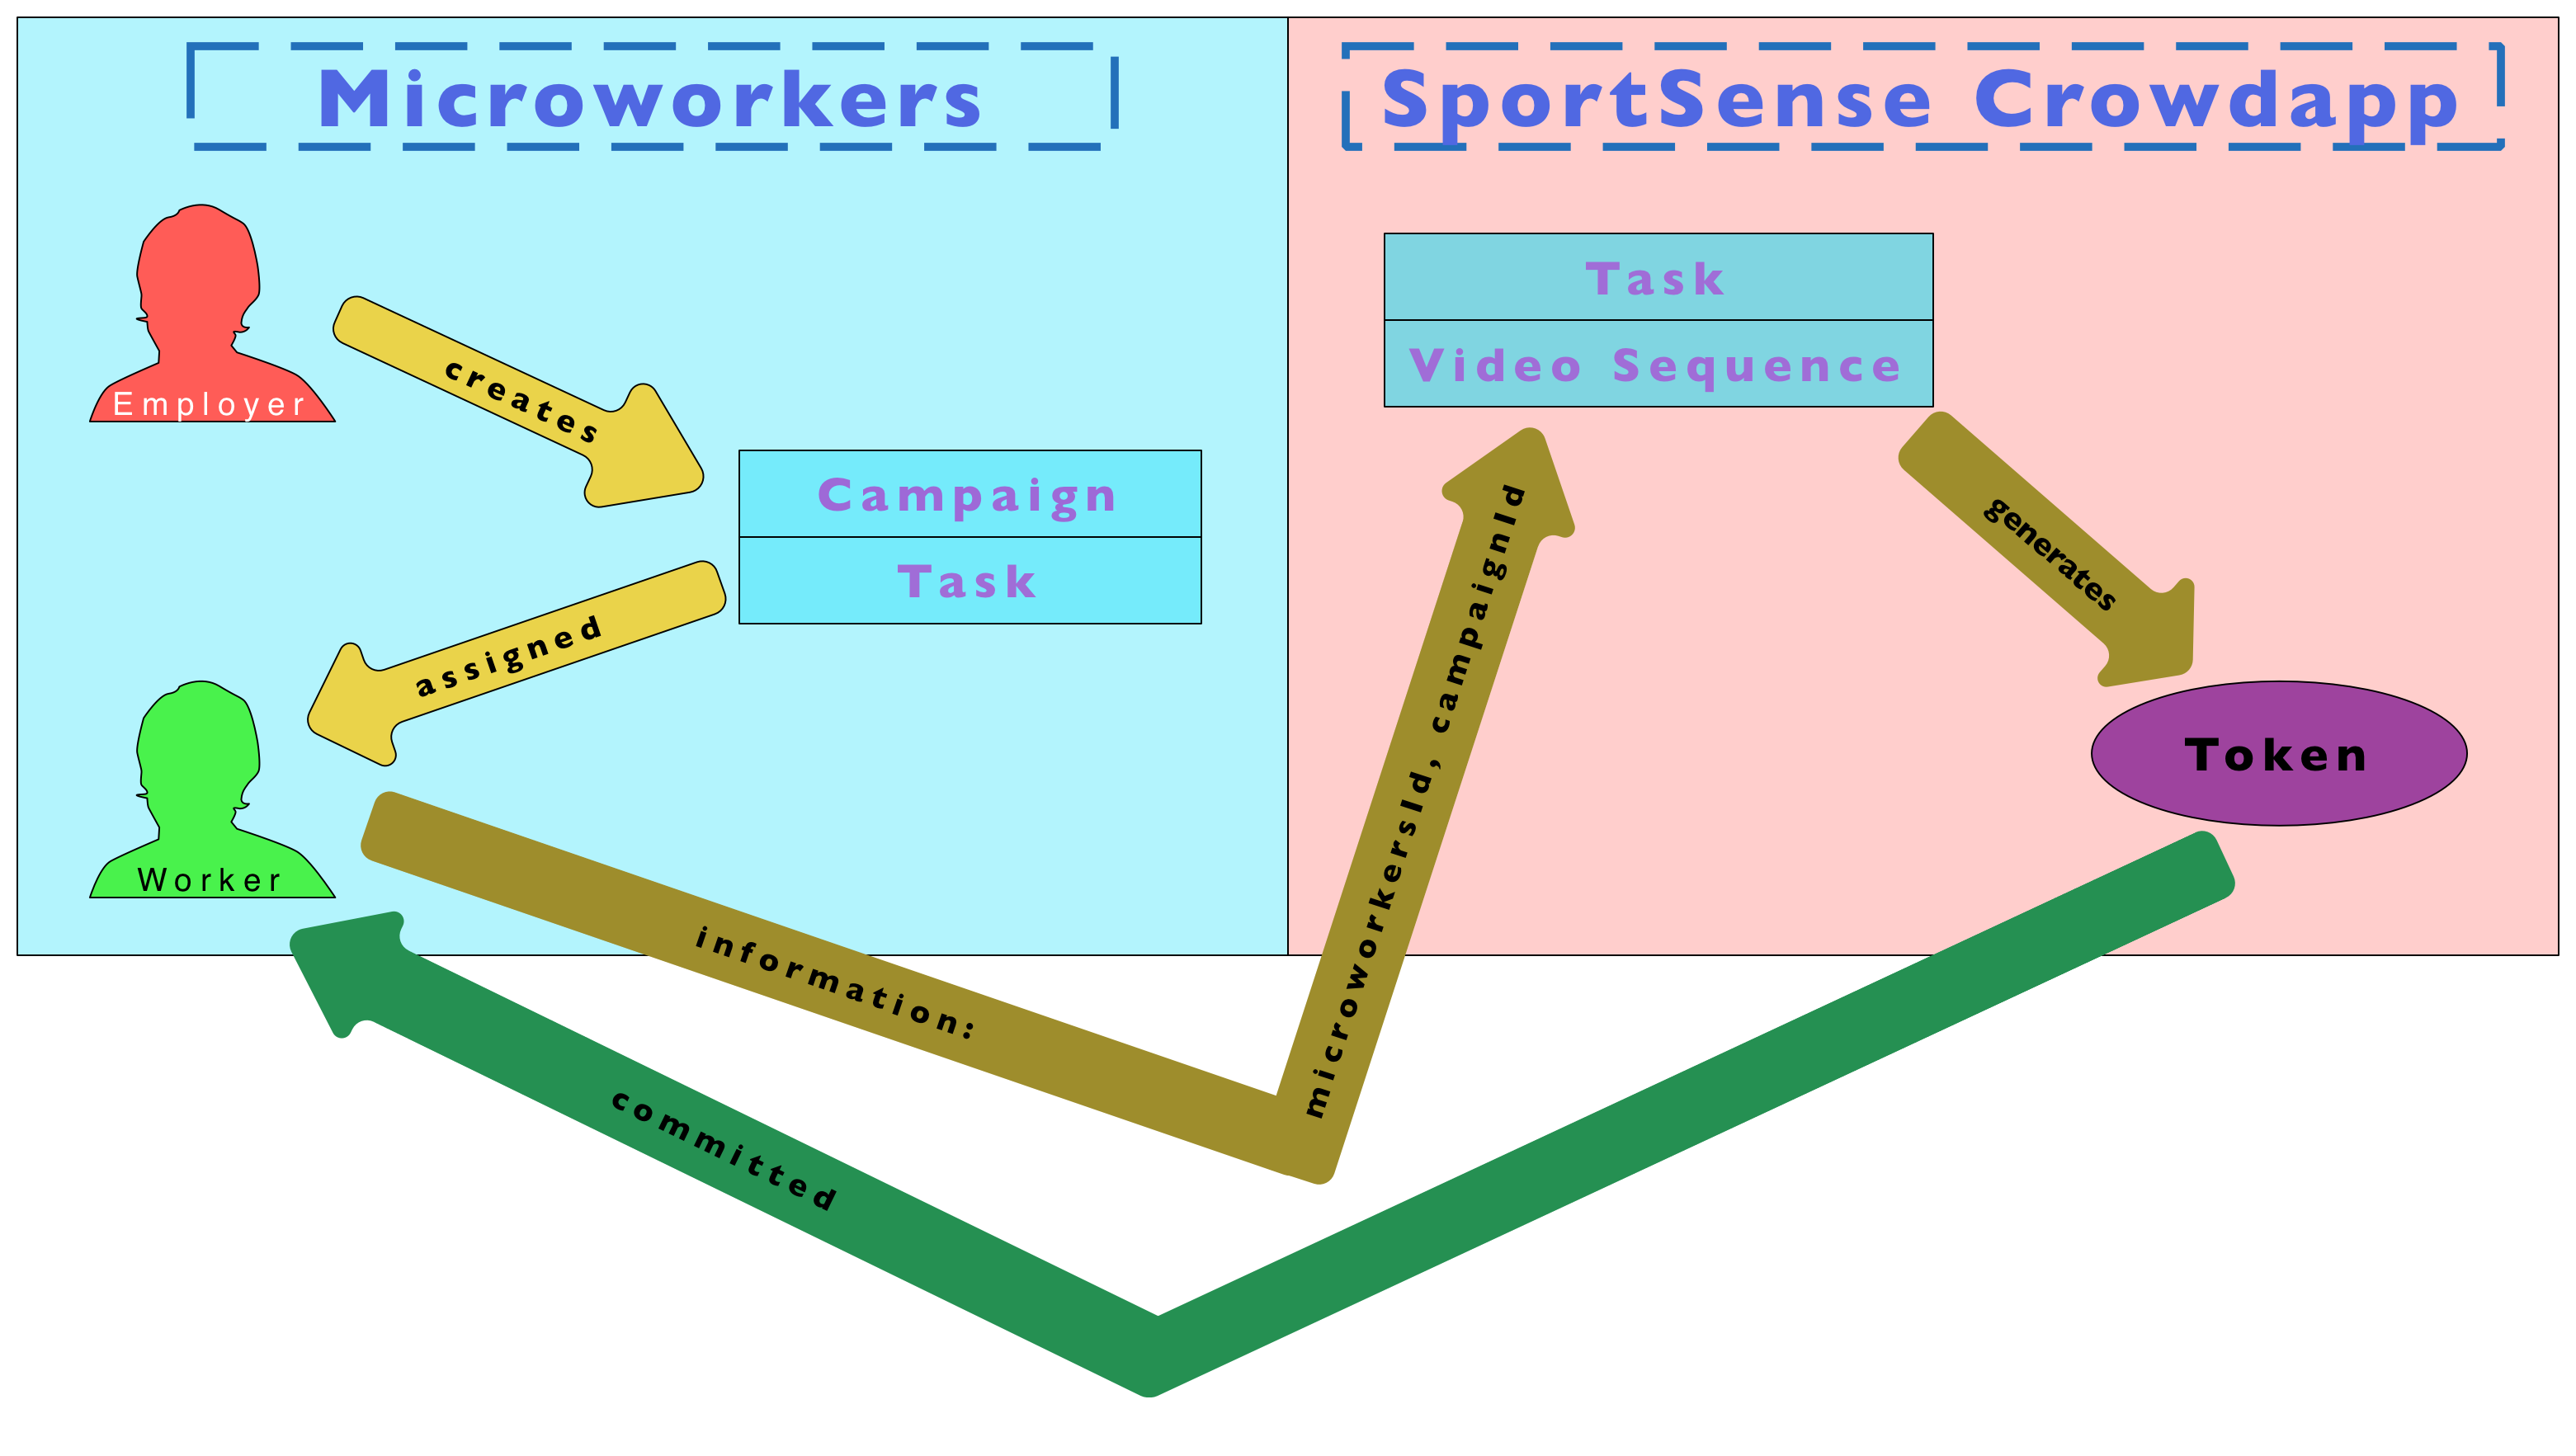
\includegraphics[width=0.9\textwidth]{Schema}
    \caption{Interaction between Microworkers and SportSense Crowdapp}
    \label{fig:Schema}
\end{figure}

Figure \ref{fig:Schema} shows the interaction between the Microworkers platform and the SportSense Crowdapp. As employer on Microworkers, users have the possibility to create campaigns containing a specific number of subtasks.

Every task on Microworkers is assigned to a worker. This worker opens the Crowdapp, where he will receive a task with a specific video sequence. With the information provided by Microworkers, his token can be generated and, after finishing the task, shown to the worker.
This token is the key that he must enter in Microworkers to complete the task and finally also receive payment. A detailed explanation what specifications we made for creating the campaign can be read in Section \ref{sec:Microworkers}.

\section{Data Model}

In this thesis, a system has been built with which new campaigns can be created easily with other tasks, and which also has the potential to be extended to other sports. The following figure describes the data model that underlies this system.

\begin{figure}
    \centering
    \hspace*{-0.15\textwidth}
    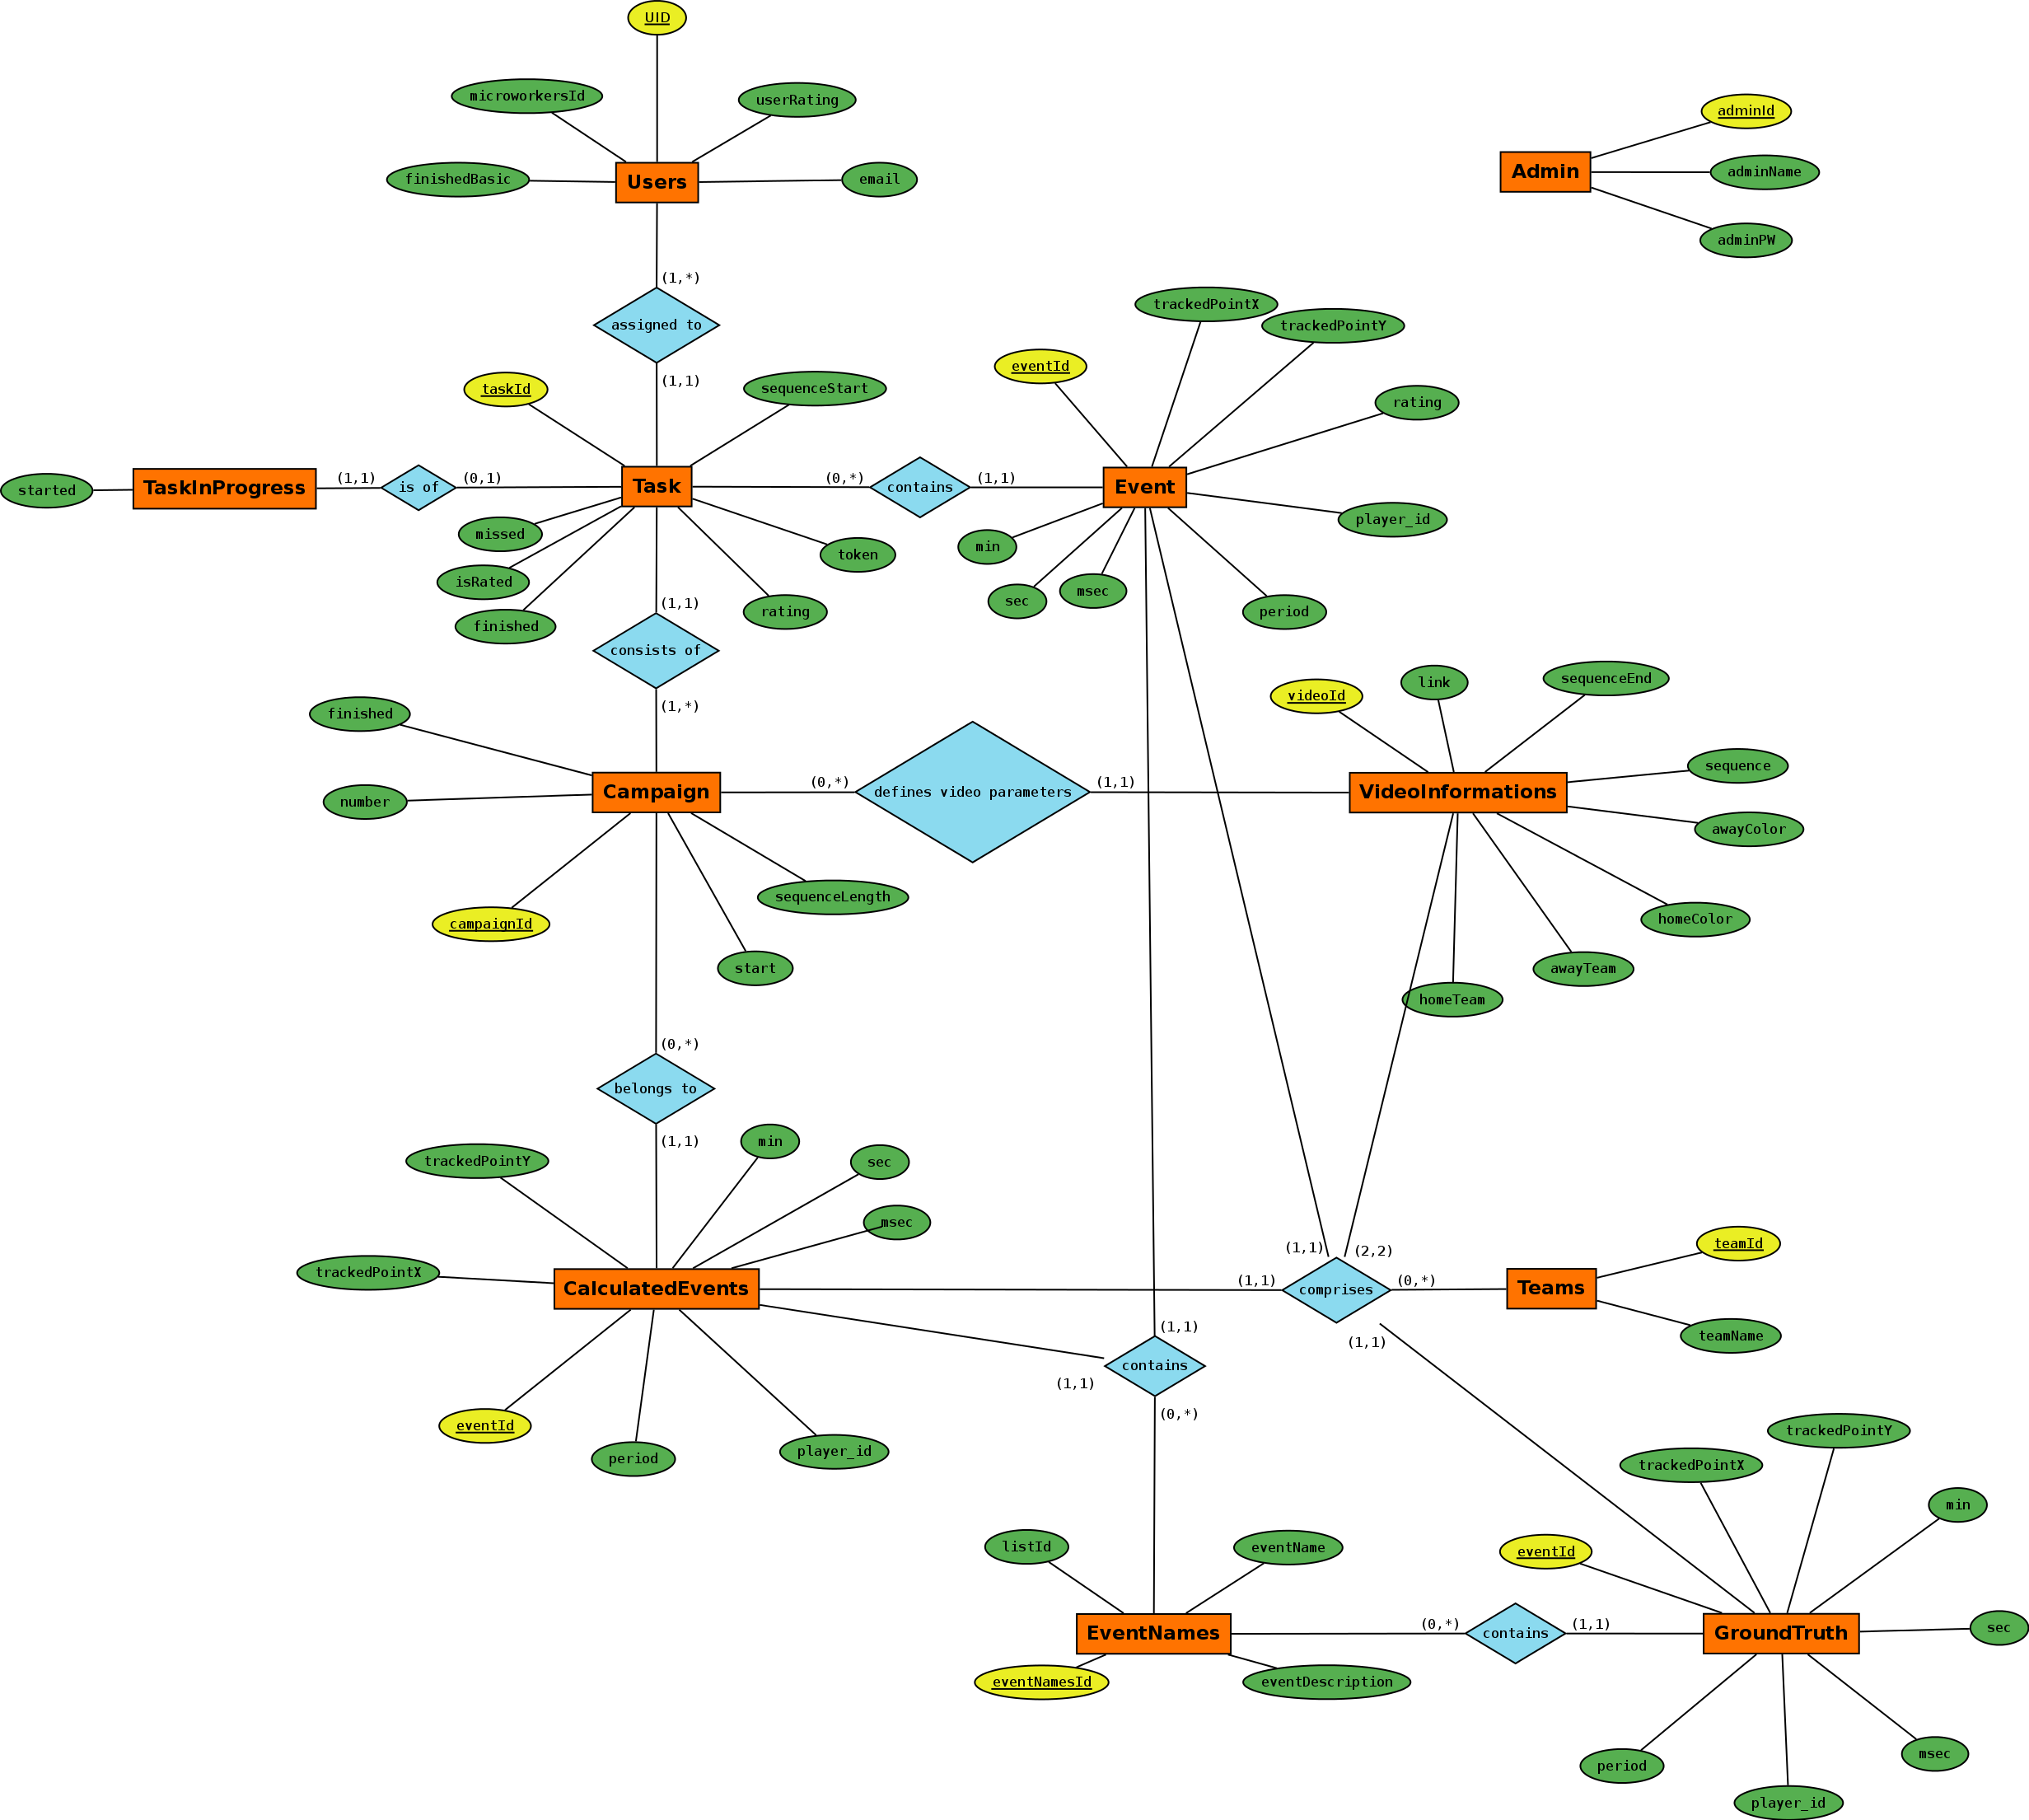
\includegraphics[width=1.3\textwidth]{ER_Diagramm}
    \caption{System data model}
    \label{fig:systemmodel}
\end{figure}

\paragraph{Admin}
The $Admin$-entity contains an identifier ($AdminId$), which holds the ID stored as a session value. For the login system, this table also holds a username ($AdminName$) and an password ($AdminPw$), which is encrypted by SHA-512.

\paragraph{Teams}
The entity “Team” stores the name of the team ($teamName$).

\paragraph{VideoInformations}

For each team ($Teams$), the entity $VideoInformations$ stores information on the team that plays at home ($homeTeam$) and the team that plays away ($awayTeam$). To help to identify the teams in the video, the color of the home team ($homeColor$) and the away team's color ($awayColor$) are also stored.
The information where a the video files is stored in the file system is saved in a relative path ($link$). 
To avoid creating campaigns with starting or ending values outside the video length, the $VideoInformations$ entity also stores the time the video starts ($sequence$) and the time the video file ends ($sequenceEnd$).

\paragraph{Campaign}
Every tuple in the campaign refers to a video $VideoInformations$, which provides the information of the video for this campaign. Every campaign starts at a position ($start$) in the video and has a specified number of tasks ($number$) to be done. To get the information on how long every temporal sequence of a task need to be, the entity $Campaign$ contains a value for this task's length ($sequenceLength$).

\paragraph{Users}
Every Microworkers user visiting the SportSense Crowdapp gets registered with a unique identifier ($UID$); the system of Microworkers also provides us their used identifier ($microworkersId$). To improve the system with a rating method, every user has a rating ($userRating$).
To detect if the user has already been evaluated in a pretest to determine the confidence of his answers, this information is stored for every user ($finishedBasic$).

\paragraph{Task}
Every existing campaign ($Campaign$) consists at least of one task. The entity $Task$ stores the informations of those tasks.
If a user ($Users$) finished a task, the values of the entity $Task$ will be updated. Thereby, the number of missed tasks ($missed$) will be calculated and the task will be marked as finished ($finished$). In addition, the token generated ($token$) by the values provided by Microworkers is stored in this entity.
A task also comprises a rating ($rating$) as calculated in Section \ref{RatingSystem}, and a value to determine if the task is already rated ($isRated$).

\paragraph{Event, CalculatedEvents and GroundTruth}
The three entities Event, CalculatedEvents and GroundTruth are very similar to each other. They all store some event information attributes, like the position data for x ($trackedPointX$) and y ($trackedPointY$), the attributes for the minute ($min$), second ($sec$) and milliseconds ($msec$), which together make up the time the event happens. All of these entities also contains the ID of the teams ($team\_id$) that performed the event ($type\_id$).
As compared to CalculatedEvents and GroundTruth, the Events entity also contains an attribute holding the event's rating ($rating$).

\paragraph{EventNames}
In the $EventNames$ entity, all captured events of the corresponding task are saved, containing the values described in the Table \ref{tb:Events}. All events have a unique identifier with the primary key. This key's values consist of the values of Manchester City's dataset.
To group them more intuitive, an attribute to order ($ListId$) them on the system was added. Every event also holds a name ($eventsName$) and a description ($eventDescription$).

\paragraph{TaskInProgress}

This entity helps the system to determine whether a task has started or not. The starting time of a task ($started$) is saved. After a specific time, these tasks are deleted in the entity TaskInProgress if they are not finished with the use of an event scheduler.


\newpage

\section{Rating System} \label{RatingSystem}

Because it is not known how good the data of user inputs are, a method to establishing the correctness of data has to be determined.
Therefore, all users are first evaluated using a ground truth to establish a first reliability rating.
\newline
After this first evaluation, users are allowed to work on real data. 
The data entered in these real tasks will be used to calculated a new basis out of all entered events with respect to the corresponding user's rating.
For all users who have participated in the campaign, the rating is calculated with the new basis.

To increase the quality of the data gathered from the Microworkers, a rating system is introduced to check the quality of their given answers.

\subsection{Events}

To specify the events that should be captured, the existing dataset serves as an orientation.

\begin{table}[H]
    \centering
    \resizebox{\textwidth}{!} {
	\begin{tabular}{p{5cm}p{14cm}}
        \textbf{Event name} & \textbf{Event description}\\
		\hhline{==}
        \rowcolor{gray!30}
        	Pass & When the player in possession kicks the ball to a teammate. Passes can be long or short but must remain within the field of play.\\ 
        	\hline
	    Pass - Offside & A player is in an offside position if: \newline- He in the opposition half. \newline - He in front of the ball. \newline - Have fewer than two opposition players between himself and the goal line when the ball is played to him by a teammate. \newline The goalkeeper counts as an opposing player in this instance.\\
        	\hline
   	    Take on & A take on is an interception where the intercepting player keeps the ball.\\
        	\hline
        \rowcolor{gray!30}
	    Foul & A foul is an unfair act by a player, which is deemed by the referee.\\
        	\hline
        \rowcolor{gray!30}
	    Out & When the whole of the ball goes over the whole of the sideline or goal line.\\
        	\hline
        \rowcolor{gray!30}
	    Corner Kick & A kick taken by the attacking team that is earned when the defending team puts the ball out of play behind the goal line.\\
        	\hline
        \rowcolor{gray!30}
	    Tackle & When a player without the ball dispossesses an opponent with it.\\
        	\hline
        \rowcolor{gray!30}
	    Interception & Intercepting the ball is winning possession of the ball as it is being passed from \newline one opposition player to another.\\
        	\hline
	    Clearance & When a defending player clears the ball out of danger. The purpose of a clearance is to relieve the pressure being exerted by the attacking team.\\
        	\hline
        \rowcolor{gray!30}
	    Shot off target & When an attacking player kicks the ball towards the goal in an effort to score and the ball misses the goal.\\
        	\hline
	    Post & When the referee chooses to allow play to continue if an offense has been made against the team in possession of the ball, he enforces the advantage rule. He does this if the attacking team would be unnecessarily penalized if play were to be stopped.\\
        	\hline
        \rowcolor{gray!30}
        	Shot on target & When an attacking player kicks the ball towards goal in an effort to score and the ball flies in direction of the target.\\
        	\hline
        \rowcolor{gray!30}
	    Goal & A goal is scored when the entire ball crosses the whole of the goal line between the goalposts and the crossbar.\\
        	\hline
        \rowcolor{gray!30}
	    Card & Used by a referee to enforce discipline in a match. A yellow card is a warning, and a player collecting two of these will be given a red card and sent from the field of play. A straight red card can be produced by a referee for a bad offense such as serious foul play or a professional foul.\\
        	\hline
	    Pass - Ball recovery & When the player in possession kicks the ball to a teammate and the other team retains it.\\
        	\hline
	    Pass - Ball touch & When the player in possession kicks the ball to a teammate by touching it only once.\\
        	\hline
    \end{tabular}
    }
   \caption[]{Events used in the system with the appropriate description, (adapted from\footnotemark)}
    
    \label{tb:Events}
\end{table}
\footnotetext{http://worldsoccer.about.com}

To reduce the difficulty level, not all of those events are used here. The events used in the system are marked with a gray background.
This was done because similar events, for example, an interception and a clearance, are to close to each other and will produce too many errors, especially by lay people evaluating football.

\subsection{Position}

The input field to let users enter position data looks like Figure \ref{img:Field} below.

\begin{figure}
    \centering
    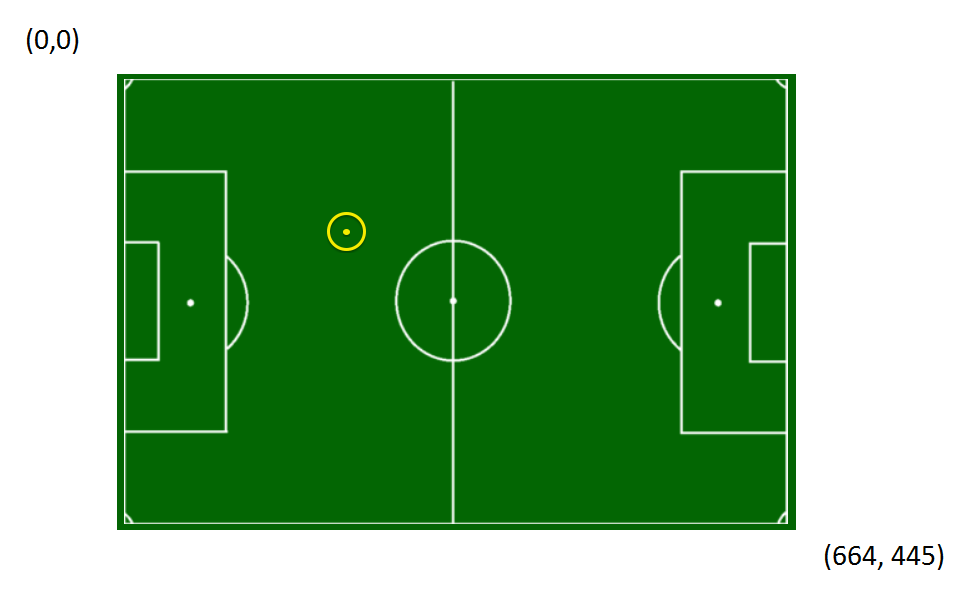
\includegraphics[width=\linewidth]{FieldCoordinates}
    \caption{Soccer field used in SportSense}
    \label{img:Field}
\end{figure}

Where the x-coordinate is 664 and the y-coordinate 445 units long.
The acceptable value to rate the users will be 40 units, which is in the diagonal distance 
$$
	\frac{40}{\sqrt{664^2 + 445^2}}*100 = 5 \%
$$
Considering that the size of a soccer field is about $90\times45$ meters, $5\%$ of the diagonal length would be about five meters long.

The yellow point and circle indicates where a user set the position. His radius is 20 units, which is at the same time the $\delta_{position}$, which is accepted and rated with 0.


\subsection{Userrating}\label{subsec:userRating}
All users start with an initial rating of 0. If a task is finished the rating of the corresponding user will be rated with his old rating plus the new one.
This entails that a user's rating is:

\begin{equation}
	R_{User}=\sum\limits^{}_{n} R_{Task}
\end{equation}

where $n$ is the number of tasks per user.


\subsection{Rating of the task}

With the rating of all events R$_{Event}$ in a task, the rating for the task will be calculated by 

\begin{equation}
	R_{Task}=\sum\limits^{}_{n} R_{Event}
\end{equation}
where $n$ is the number of events per task.


\subsection{Rating of the event}

If a user's rating $\delta_{user}$ is smaller than $-1$, he will receive a warning.
If the user's rating is smaller than $\delta_{user} \le -1.5$, the user will not be able to do any more tasks in the SportSense Crowdapp.


Every input will be rated using a ground truth at the beginning. This rating of the event is defined as the sum of the rating of all dimensions of an event, as we show in Equation \ref{eq:ratingEvent}.
\newline

This section defines all values of the basis without a tilde ($\backsim$) and all user-entered data points with a tilde.

\begin{equation}\label{eq:ratingEvent}
	R_{Event}=\frac{R_{T}+R_{P}+R_{E}+R_{t}}{4}
\end{equation}
$$R_{Event} \in [0,1]$$

where R$_{T}$ is the rating of time, R$_{P}$ is the rating of the position, R$_{E}$ is the rating of the event and, R$_{t}$ is the rating of the team. The parts of the total rating will be discussed in the following.

\paragraph{Rating of the team R$_{t}$}
To get the value for the team R$_{t}$, we compare the entered team's ID against the basis team identifier.

\begin{equation}
	R_{t} =
	\begin{cases}
		1	& \text{if team} =  \widetilde{team}\\
		0	& \text{if team} = \widetilde{team} \\
   \end{cases}
\end{equation}


\paragraph{Rating of the event R$_{E}$}
To evaluate if the user entered the right or wrong event, we compare his event ID with the basis events identifiers.

\begin{equation}
	R_{E} =
	\begin{cases}
		1	& \text{if event } =  \widetilde{event}\\
		0	& \text{if event } = \widetilde{event} \\
   \end{cases}
\end{equation}



\paragraph{Rating of the position R$_{P}$}

A measure for the distance of the user data is given by position $X$ and position $Y$.
The rating on the position data is done by calculating the Euclidean distance (L2) between the point set by the user and the point given in the ground truth.

\begin{equation}
	D_{points} =\sqrt{(X - \widetilde{X})^2 + (Y - \widetilde{Y}) ^2}
\end{equation}
\\

If the distance between the basis($\widetilde{X}$, $\widetilde{Y}$) and the data entered by the user (X, Y) D$_{position}$ is less than the threshold value $\delta_{position} = 20$, the rating is squared to reward users, adding a small positional difference.

\begin{equation}
    R_{P} = (\frac{D_{points}}{\delta_{position}})^2
	\label{eq:DistanceRatingSmall}
\end{equation}
\\


if the distance t is bigger than $\delta_{position}$ the rating of the distance is calculated the following linear function:

\begin{equation}
    R_{P} = \frac{D_{points}}{\delta_{position}}
    \label{eq:DistanceRatingBig}
\end{equation}


With Equations \ref{eq:DistanceRatingSmall} and \ref{eq:DistanceRatingBig}, the rating for the distances will result in:

\begin{equation}
	R_{P} =
	\begin{cases}
		\frac{D_{points}}{\delta_{position}}	&	D_{points} > \delta_{position} \\
		(\frac{D_{points}}{\delta_{position}})^2 &	D_{points} \le \delta_{position}
	\end{cases}
\end{equation}

\begin{figure}[H]
    \centering
    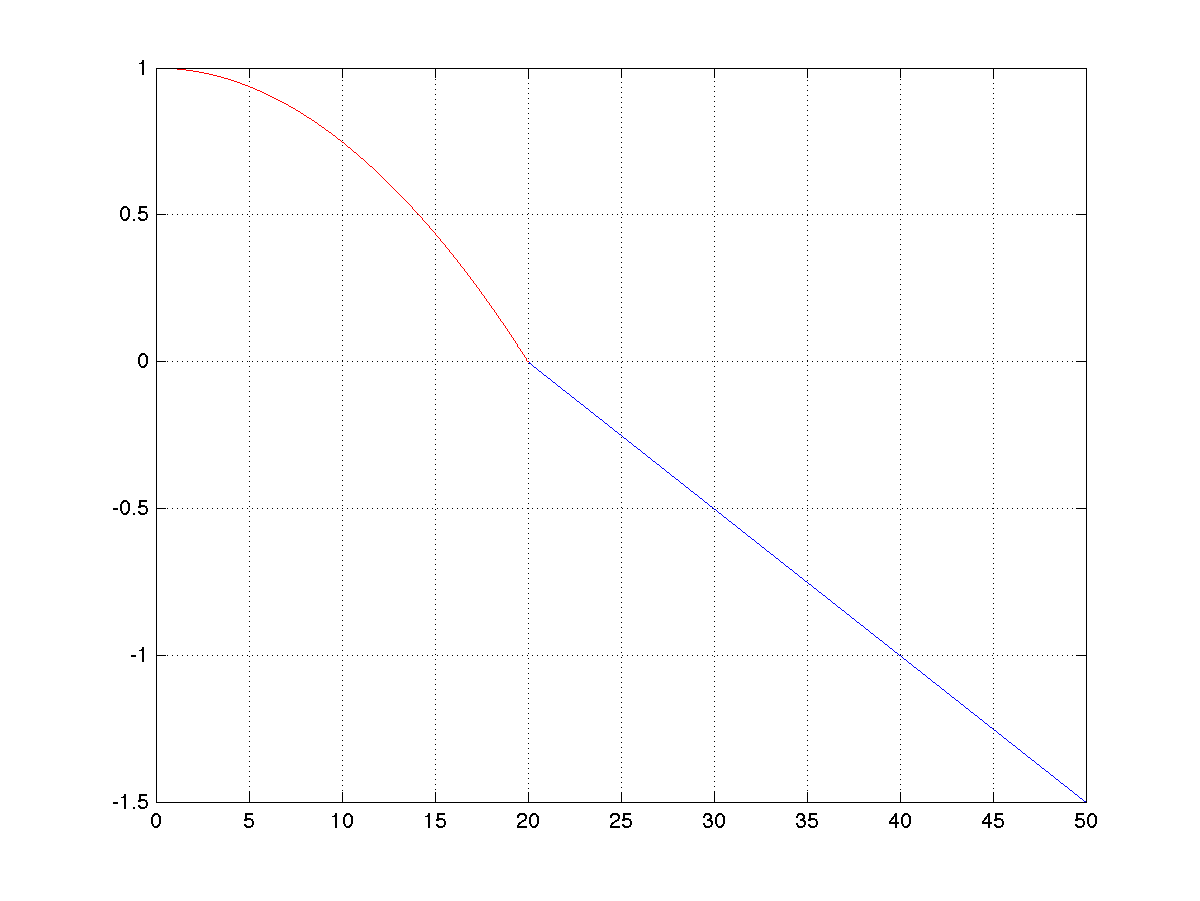
\includegraphics[width=0.8\textwidth]{DistanceCalculationPlot}
    \caption{Distance calculation of position}
    \label{fig:distPos}
\end{figure}

Figure \ref{fig:distPos} displays the function R$_{P}$ graphically. With this differentiation of the distance calculation, the rating of position of points with a small distance to the ground truth points can be kept small, because it is almost impossible to enter the exactly same position twice, and all points with a bigger position distance than $\delta_{position}$ are rated linear.

\paragraph{Rating of the time R$_{T}$}

To calculate the rating for the difference in the time compared to the ground truth, sharp boundaries are set for the accepted values. This gives:

\begin{equation}
	R_{T} =
	\begin{cases}
		1	& if D_{time} = 0.0s \\
		0	& if D_{time} = 0.5s \\
		-1	& if D_{time} = 1.0s \\
   \end{cases}
\end{equation}

Where the distance between the times is calculated by:
 $$ D_{time} = |time| - |\widetilde{time}|$$

To calculate the rating of the time for a point against the ground truth point, a linear function:

\begin{equation}
	R_{T} = 1 - 2 * D_{time}
\end{equation}

\newpage


\section{Data Integration}

By using the user's rating as calculated by the pretest in Section \ref{subsec:userRating}, a new basis is calculated with the entered data.
This section presents two different methods to calculate the basis. In Section \ref{subsec:UPGMA} we first introduce an integration and cleaning method based on the unweighted pair group method with arithmetic mean (UPGMA) algorithm. Section \ref{DBSCAN} presents a density-based clustering algorithm.

\subsection{Distance calculation}\label{sec:Dist_calc}

For both algorithms, the difference between two entered events needs to be calculated.
The mathematical approach to calculate the difference between two data-points in the system will be described. Each data-point is considered as a vector in a five-dimensional space, with the dimensions time, position of $X$ and $Y$, event and team. For each vector, the following distance functions are defined.

The difference between two entries ($E1$, $E2$) is calculated by the arithmetic mean over all attributes of the points:

\begin{equation}\label{eq:Distance_points}
	D_{E1,E2}=\frac{D_{P} + D_{T} + D_{t} + D_{E}}{4}
\end{equation}

where D$_{T}$ is the difference of the time, D$_{P}$ is the difference of the position, D$_{E}$ is the difference of the events, and D$_{t}$ is the difference of the team. Those parts of our difference calculation are described hereafter.
\newline


Where the respective distances are calculated by:

\paragraph{Difference in positions D$_{P}$}
$$		D_{P}= \frac{\sqrt{(X_{E1} - X_{E2})^2 + (Y_{E2} - Y_{E2})^2}}{\delta_{position}}
$$		
		
\paragraph{Difference in time D$_{T}$}

$$		D_{T} = |time_{E1} - time_{E2}| $$

\paragraph{Difference in teams D$_{t}$}
$$		D_{t} =
		\begin{cases}
			1	& \text{if team$_{E1}$ } = \text{ team$_{E2}$} \\
			0	& \text{if team$_{E1}$ } = \text{ team$_{E2}$} \\
		\end{cases}
$$

\paragraph{Difference in events D$_{E}$}
$$		D_{E} =
		\begin{cases}
			1	& \text{if team$_{E1}$ } = \text{ team$_{E2}$} \\
			0	& \text{if team$_{E1}$ } \neq \text{team$_{E2}$} \\
		\end{cases}
$$

With this difference calculation, two exact same events will end up with 
$$E1 \equiv E2 \qquad \Rightarrow \qquad D_{E1,E2}=0$$

\subsection{Unweighted pair group method with arithmetic mean}\label{subsec:UPGMA}

The first way to calculate the bases uses the ideas of unweighted pair group method with arithmetic mean (UPGMA) \cite{Sokal:1958}. The basic approach of the algorithm is to join the two clusters with the smallest distance to a new one, until only one cluster is left, which will be the root of the three.
The distance between all points is calculated by the distance calculation between two points in this project, as described in Section \ref{sec:Dist_calc}.

UPGMA, is a hierarchical clustering algorithm starting at the bottom for creating phylogenetic trees, was initially designed for the use in protein electrophoresis. The requirements of the algorithm is the distance between each pair of the data set.

The algorithm starts with an unresolved tree and joins the two closest points until only one point is left.

This approach does not want to join all points until only one single point is left. A value is set for the maximum distance two points are allowed to have to join them. With this change, this will be stopped if the distance between two clusters is bigger than the specified threshold.


The new point is calculated by two points $E1$ and $E2$, as in the following equations.
All variables with a circumflex(\^{}) belong to the second event and all variables without one belong to the first event.

The variable $R$ is the rating of the point, $t$ stands for the team, $T$ for the time, and $X$ and $Y$ for the corresponding position of each event.

new positionX:
$$
positionX_{E1,E2} = \frac{X * R + \hat{X} * \hat{R}} {R + \hat{R}}
$$


new positionY:
$$
positionY_{E1,E2} = \frac{Y * R + \hat{Y} * \hat{R}} {R + \hat{R}}$$

new time:

$$
time_{E1,E2} = \frac{T * R + \hat{T} * \hat{R}} {R + \hat{R}}$$


new team:

$$
team_{E1,E2} =
		\begin{cases}
			t	& \text{if} \enskip R  \enskip \ge \enskip \hat{R} \\
			\hat{t}	& \text{if} \enskip R \enskip < \enskip \hat{R} \\
		\end{cases}
$$

new event:

$$
event_{E1,E2} =
		\begin{cases}
			E	& \text{if} \enskip R \enskip \ge \enskip \hat{R} \\
			\hat{E}	& \text{if} \enskip R \enskip < \enskip \hat{R} \\
		\end{cases}
$$

After calculating the new row composed by two events, those events are deleted from the data list and the new event added.
For this new event, the distance to all other events is again calculated.
This is done until there are no more events with a distance smaller than one.

\paragraph{Algorithm}

Listing \ref{lst:UPGMA} presents the pseudocode, showing the calculation of the UPGMA method.
As described below, the distance between all points in the dataset $data$ is calculated and stored in a matrix $distanceMatrix$. A counter array $counter$ is also created, containing ones for the size of the dataset, because every data entry consists of exactly one point at the beginning.


As long as $distanceMatrix$ exhibits values smaller than $1$, the closest two data-points are joined to a new point. The closest ones are those ones with the smallest values in the distance matrix. After calculating the new point from those two points with respect to their rating, those two points points are deleted from $data$ and the new point is added. The ratings of the two points is also removed and a new entry is added to the rating array containing the sum of the two points ratings. 
After joining to points, the $counter$ also need to update by the amount of the two joined point's rating.
At least, the new distance of the two joined points to all others is calculated and the $distanceMatrix$ updated.

In the end, all points existing in the data with a counter bigger than 4 are accepted, which means that all accepted points need to be calculated out of more than four points.

\begin{lstlisting}[caption={Algorithm joining all points similar two each other},label={lst:UPGMA}]
FUNCTION calculatePoints(data, rating)
	distMatrix = getDistMatrix(data);
	counter = ones array with length of rating;
	
	WHILE distMatrix contains elements <=1
		[index1, index2] = smallest value in distMatrix;
		
		newRow = calculate the new datapoint with the elements index1, index2;
		data[lastRow+1] = newRow;
		
		rating[lastRow+1] = rating[index1] + rating[index2];

		counter[lastRow+1] = counter[index1] + counter[index2];
		
		newDist = calculate the distance of the newRow to all others;
		distMatrix[lastRow+1] = newDist;

	END WHILE

	RETURN data = data where appropriate counter>=4
END FUNCTION
\end{lstlisting}

To get the distance matrix, for each row the distance to all other rows in the dataset is calculated. The distance between two rows is calculated as described in Equation \ref{eq:Distance_points}.
After calculating all values, an upper triangular matrix is returned.

\begin{lstlisting}[caption={Algorithm to calculate the distance of two points}]
FUNCTION getDistMatrix(data)
	FOR I = 1 to length of data
		FOR J = I + 1 to length of data
			Dist = calculate the distance of point I and J;
			DistMatrix(I, J) = Dist;
		END FOR
	END FOR
	RETURN DistMatrix;
END FUNCTION
\end{lstlisting}

\subsubsection{Discussion}

The main problem of our UPGMA approach is that it gives more weight to the first point in the list; thus, when joining the two closest events, the event with the corresponding higher rating will prevail. However, this leads to a propagation of errors if the first entered event type or team with the bigger rating was wrong, because the new event joined out of two events gets also a rating that is the sum of the two old ratings.



\subsection{DBSCAN}\label{DBSCAN}

The second method is to use a cluster method that starts from an unknown distribution of the data.
For this purpose, the DBSCAN algorithm is used. DBSCAN is a density-based algorithm to cluster the data and detect outliers. The idea of the DBSCAN algorithm is that for each point in a neighborhood with distance $\epsilon$ there has to be a minimum number of points($MinPoints$), to be accept as a cluster.
DBSCAN is able to distinguish between different types of reachability.

In the DBSCAN algorithm, different kinds of points related to a cluster exist \cite{ester:1996}, as described below:


\paragraph{Directly density reachable}
All points with a distance $D(p,q) \le \epsilon$ are density reachable for point p.

\paragraph{Core and border points}
If a point is density reachable, there are two possible states a point can get. A point is a core point if it satisfies that the point itself has more density reachable points than $MinPoints$.
$\# D(p,q_{i}) \le \epsilon \ge MinPoints$ where i is one element of the data $ p_{i} \neq q$

\paragraph{Density-reachable}
A point p is density-reachable from a point q if it there exists a chain of density connected points including the points p and q.

\paragraph{Density-connected}
A point p is density-connected with a point q if there exists a point r such that p is density-reachable from r and also q is density reachable from r.

\paragraph{Cluster}
A cluster with respect to $\epsilon$ and $MinPoints$ is a non-empty subset of data satisfying the conditions
\begin{itemize}
    \item $\forall p,q $ if $p \in C$ and $q$ is density recheable from p wrt. $\epsilon$ and $MinPoints$ than $q \in C$, where C is a cluster.
    \item $\forall p,q \in C$ the points $p$ and $q$ are density-connected wrt. $\epsilon$ and $MinPoints$. 
\end{itemize}

\paragraph{Noise}
A point is marked as noise if it do not belong to a cluster where clusters are built with respect to $\epsilon$ and $MinPoints$.
\newline

In our approach the calculation does not differentiate between density-reachable and density-connected points, because by setting a different $\epsilon$ and $\epsilon_{2}$ for the density-connected points the number of density-connected points can be reduced.

\begin{figure}
    \centering
    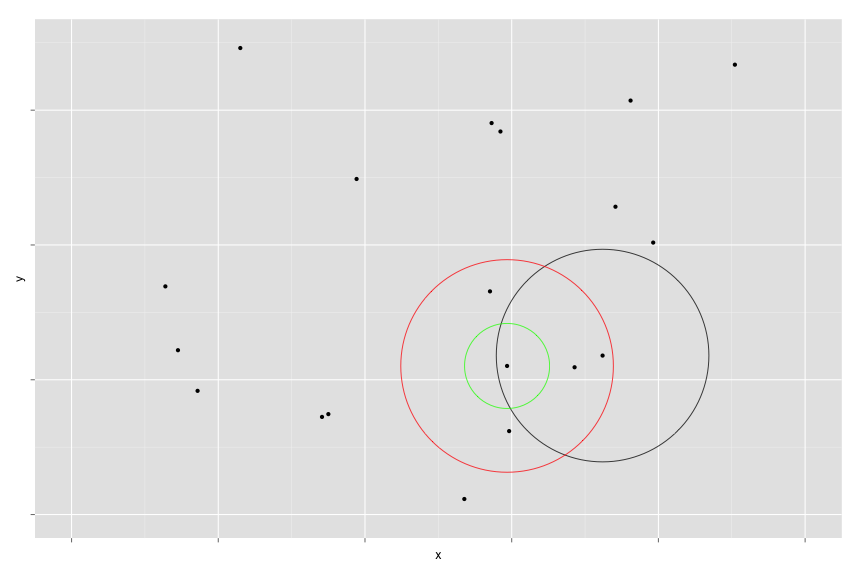
\includegraphics[width=0.8\textwidth]{DBSCAN_distance}
    \caption{Reachability of DBSCAN}
    \label{fig:DBSCAN_distance}
\end{figure}

Figure \ref{fig:DBSCAN_distance} shows that, with decreasing the $\epsilon_{1}$ towards $\epsilon_{2}$ the chain can be brought to stop at some point. 
When starting with the first point in the black epsilon, one gets three density-reacheable points with it.
If one would continue with $\epsilon_{1}$, as illustrated with the red color, one would create a big chain with two new points points in it.
By lowering the setting for $\epsilon_{1}$ to $\epsilon_{2}$ for density-reachable points, one can decrease the number of density-connected points.

As previously, to calculate the distance of two points the calculation in Section \ref{sec:Dist_calc} is used.

\paragraph{Algorithm}

The clustering method with the DBSCAN starts by setting the cluster counter to 0.
For each row in the dataset, the distance to all other rows in the dataset is calculated, starting starting with the first row.
If there are more than the minimum number of points required to build a cluster, the cluster gets expanded and increase the cluster counter by one, to create a new cluster.
If the number of indexes with a value smaller than $\epsilon_{1}$, the data point is an outlier and is tagged as noise by setting its class to $-1$.

If the number of points similar to it is bigger than one and smaller than $minPoints$, this point is marked as not clustered.


\begin{lstlisting}[caption={Algorithm for the DBSCAN method},label={lst:DBSCAN}]
FUNCTION DBSCAN(data, MINPOINTS, EPS1, EPS2)
	clusterNumber = 0;
	FOR each row in the dataset data
		Dist = calculateDistance(row, data);
		ind = all Distances > EPS1;
		IF size(ind) > MINPOINTS
		    class(ind) = clusterNumber;
			expandCluster(data, ind, clusterNumber, EPS2);
			clusterNumber++;
		ELSE IF	size(ind) == 1
			class(i) = -1;
		ELSE
			class(i) = 0;		
		END IF
	END LOOP
	RETURN class;
END FUCTION
\end{lstlisting}


To expand a cluster in Listing \ref{lst:DBSCAN} we use the vector containing all values which belong to this cluster.
For each index in the vector we calculate the distance to all other points. The new calculated distances will be compared to $\epsilon_{2}$. If the number of values smaller than $\epsilon_{2}$ is bigger than one, those indices are added to the same class.
This is done recursively until there are no more points density-connected.

\begin{lstlisting}[caption={Algorithm to expand cluster}, label={alg:expandCluster}]
FUNCTION expandCluster(data, ind, clusterNumber, EPS2)
	WHILE Ind is not empty
		row = data(ind(1));
		Remove ind(1);
		dist = calculateDistance(row, data);
		ind1 = all Distances > EPS2;
		IF size(ind1) > 1
			class(ind1) = clusterNumber;
			expandCluster(data, ind1, clusterNumber, EPS2);
		END IF
	END WHILE
END FUNCTION
\end{lstlisting}

The function $calculateDistance$ in Algorithm \ref{alg:expandCluster} calculates the distance between one row and all other data rows in the dataset. The distances are calculated as described in Section \ref{sec:Dist_calc}.
After calculating all distances, the arithmetic mean of all distances in all dimensions is calculated.
\newline

For each data point, the introduced algorithm calculates its corresponding class. Furthermore, the algorithm also marks the points that are considered as noise.
To calculate the base, all points marked as noise are removed.
The position and time of the new base is then calculated by the arithmetic mean of all positions and times corresponding to the cluster with respect to the workers rating.
The majority of all events in the cluster set the event and team value of each basis.



\subsubsection{Discussion}
The problem of the DBSCAN algorithm is that it also accept density-connected points.
Those density-connected points are specially denoted in an array containing the types of a point. This number of density-connected points can be reduced by $\epsilon_{2}$.
The average runtime complexity of DBSCAN is $O(n \log n)$, where n is the data set length. But the complexity is not an disqualifier in our application, because the clustering and calculation of these basis events happens offline in perspective to the user entering the data.
A disadvantage of DBSCAN is that it is not deterministic, border points can be reached from multiple clusters, and the calculation of the clusters depends on the chronology of the entered points.
